\chapter{Recurrent Neural Networks (RNN)}

A recurrent neural network (RNN) is a class of artificial neural network where connections between units form a directed cycle. This creates an internal state of the network which allows it to exhibit dynamic temporal behavior. Unlike feedforward neural networks, RNNs can use their internal memory to process arbitrary sequences of inputs. This makes them applicable to tasks such as unsegmented connected handwriting recognition or speech recognition.

\begin{figure}[h]
  \centering
  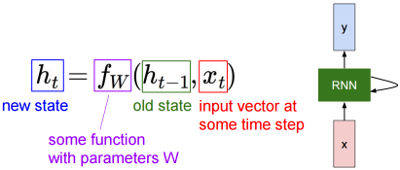
\includegraphics[width=0.4\textwidth]{Images/recurrent_neural_networks/1.png}
  \caption{RNN}
\end{figure}

Notice that the same function and the same set of parameters are used at very time step!
We can not have RNNs of enormous length because we have to store in memory the hidden state of each time step to be able to back-propagate. Normally we will have RNNs of max ~25 length.  To process bigger sequences we will divide the sequence in chunks of ~25 and the last hidden state of a chunk is the initial hidden state of the next chunk.

Let's see some wire examples (fig~\ref{fig:rnn_examples}):
\begin{figure}[h]
  \centering
  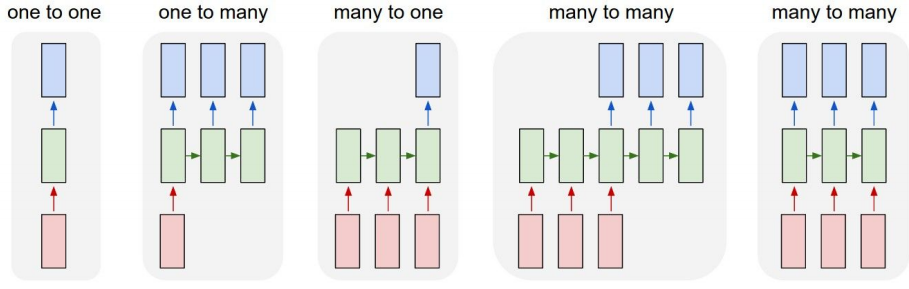
\includegraphics[width=0.8\textwidth]{Images/recurrent_neural_networks/2.png}
  \caption{RNN examples}
  \label{fig:rnn_examples}
\end{figure}
\begin{enumerate}
\item Vanilla Neural Networks
\item Image Captioning (image to sequence of words)
\item Sentiment Classification (sequence of words to sentiment)
\item Machine Translation (seq of words to seq of words)
\item Video classification on frame level
\end{enumerate}

We can stack RNNs together to produce deeper RNN. In figure \ref{fig:RNN_toghether} case we have stack 3 RNNs. It still works the same as before but now we have 3 weights.
\begin{figure}[h]
  \centering
  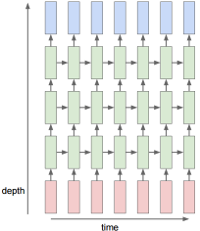
\includegraphics[width=0.3\textwidth]{Images/recurrent_neural_networks/4.png}
  \caption{Stacked RNNs}
\end{figure}

\subsection*{Practical Example}

Lets create a RNN that given a sequence of characters predicts the next one. The output is always the prob of each letter in the vocabulary to be the next character:
\begin{itemize}
\item Vocabulary: [h,l,e,o]
\item Example training sequence: "hello"
\end{itemize}

For this example we will use a Vanilla RNN:
\begin{equation}
h_t = \tanh(W_{hh}h_{t-1}+W_{xh}x_t)
\end{equation}
\begin{equation}
y_t = W_{hy}h_{t}
\end{equation}
\begin{equation}
h_0 = 0
\end{equation}

\begin{figure}[h]
  \centering
  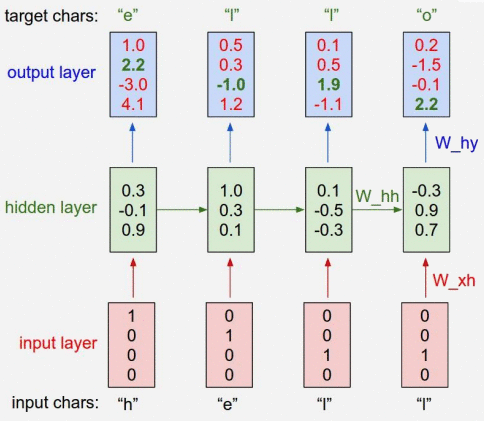
\includegraphics[width=0.5\textwidth]{Images/recurrent_neural_networks/10.png}
  \caption{Practical example. You can see this blue boxes being softmax classifier, in other words, at each time step there is a softmax classifier.}
  \label{fig:RNN_toghether}
\end{figure}

A 100 lines of code implementation of a character recognition in python is implemented here:
https://gist.github.com/karpathy/d4dee566867f8291f086

\subsection*{Image Captioning}
Example using RNN for image captioning
\begin{figure}[h]
  \centering
  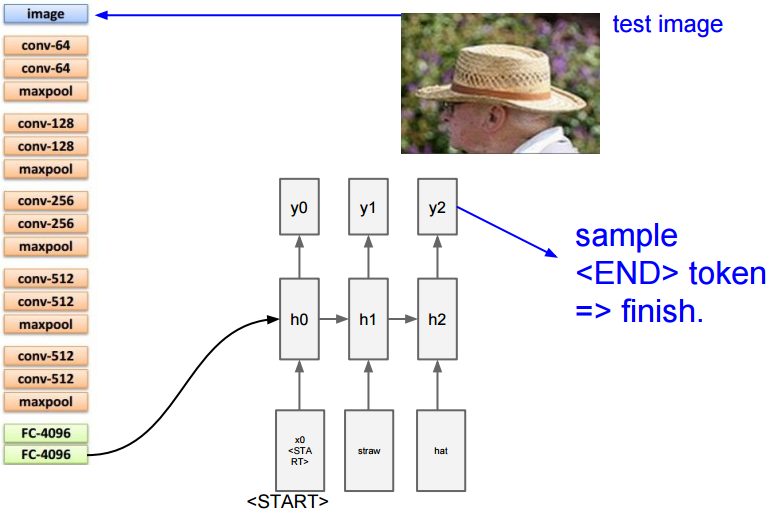
\includegraphics[width=0.5\textwidth]{Images/recurrent_neural_networks/6.png}
  \caption{"Deep Visual-Semantic Alignments for Generating Image Descriptions", Karpathy and Fei-Fei}
\end{figure}

\section{LSTM}
Normally we will not use Vanilla RNNs, instead, all papers use LSTM. It is very similar, it stills take into account the input and the last state but now the combination of both is more complex and works better. With RNN we have one vector $h$ at each time step. But with LSTM we have two vectors at each time step $h_t$ and $c_t$. Moreover in RNNs the repeating module only has one layer, \textit{tanh}. Instead, LSTM has four.

\begin{figure}[ht]
  \centering
  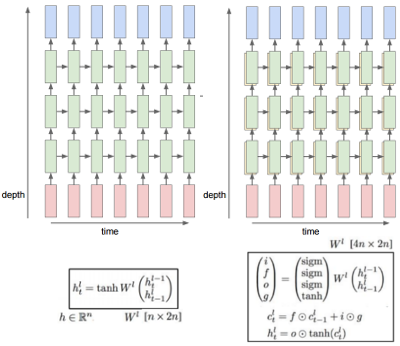
\includegraphics[width=0.65\textwidth]{Images/recurrent_neural_networks/18.png}
  \caption{\textbf{Left}: RNN with h(green), \textbf{Right}: LSTM with h(hidden vector, green) and c (cell state vector, yellow) }
\end{figure}

\subsection*{How do they work?}
\begin{figure}[h]
  \centering
  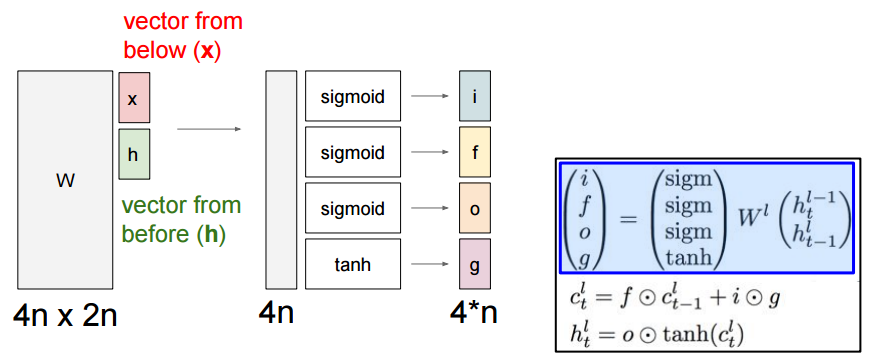
\includegraphics[width=0.65\textwidth]{Images/recurrent_neural_networks/9.png}
  \caption{LSTM first equation diagram}
\end{figure}
 where:
\begin{itemize}
\item $c$ cells. Are best though as counters
\item $h$ hidden states
\item $h_t^{l-1}$ vector from below of size $n \times 1$ ($x$ in the figure)
\item $h_{t-1}^{l}$ vector from before of size $n \times 1$ ($h$ in the figure)
\item $i \in [0,1]$ to chose if we want to add, or not, to a cell
\item $f \in [0,1]$ forget gate to reset cells to $0$
\item $o \in [0,1]$ to choose which cells are used to produce
\item $g \in [-1,1]$ to add $-1$ or $1$ to a cell
\end{itemize}

The key to LSTMs is the cell state, the horizontal line running through the top of the diagram. The cell state is kind of like a conveyor belt. It runs straight down the entire chain, with only some minor linear interactions. It’s very easy for information to just flow along it unchanged. The LSTM does have the ability to remove or add information to the cell state, carefully regulated by structures called gates.

Think of $i,f,o$ as boolean variables, we want them to have an interpretation like a gate. They a result of a sigmoid to make them differentiable. They allow us to reset and add to counters, as well as to choose what cells should be used to update $h^l_t$. We can do two operations to cells (counters):
\begin{itemize}
\item reset them with $f \odot c^l_{t-1}$
\item add -1 or 1 with $i \odot g$
\item choose what cells should be used with $o$ to update $h^l_t$: $o \odot \tanh(c^l_t)$
\end{itemize}

\begin{figure}[h]
  \centering
  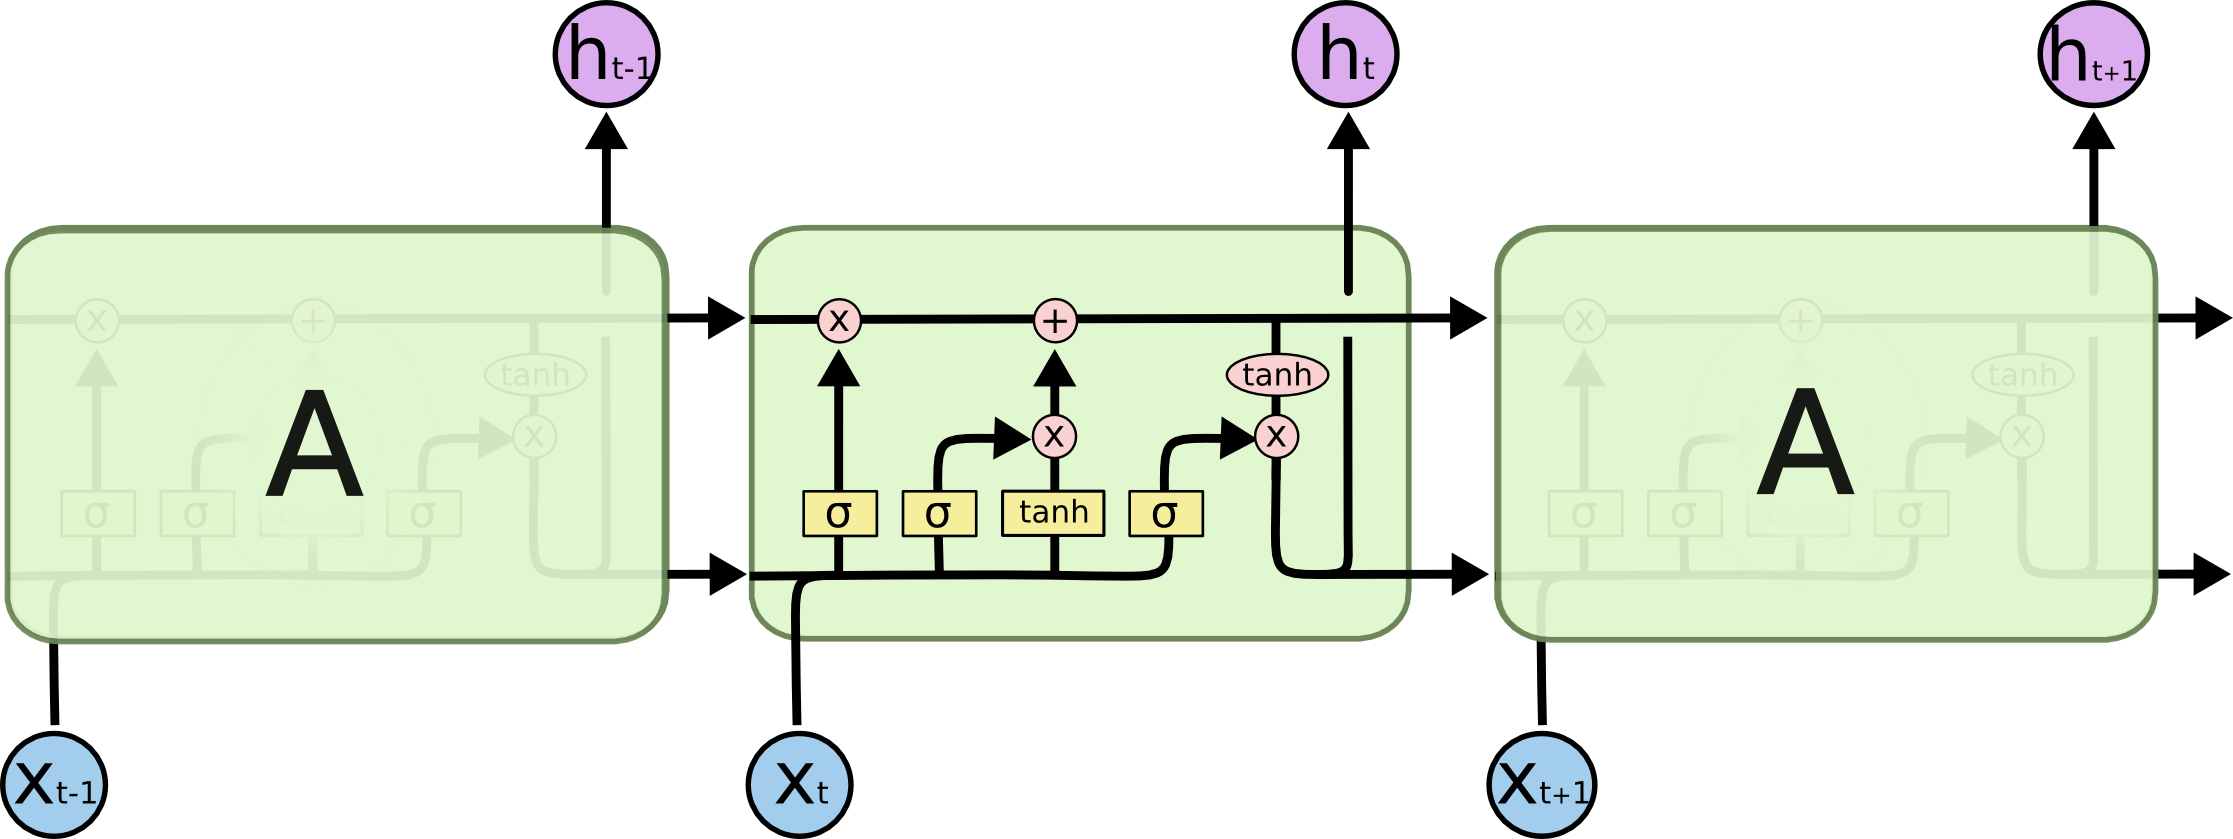
\includegraphics[width=0.65\textwidth]{Images/recurrent_neural_networks/24.png}
  \caption{LSTM diagram}
\end{figure}

\subsubsection*{Step by step}
\paragraph*{First} Decide what information we’re going to throw away from the cell state. This decision is made by a sigmoid layer called the ``forget gate layer.” It looks at $h_{t−1}$ and $x_t$, and outputs a number between $0$ and $1$ for each number in the cell state $C_{t−1}$. A $1$ represents ``completely keep this” while a $0$ represents ``completely get rid of this.” For example, in a language model trying to predict the next word based on all the previous ones the cell state might include the gender of the present subject, so that the correct pronouns can be used. When we see a new subject, we want to forget the gender of the old subject.

\begin{figure}[h]
  \centering
  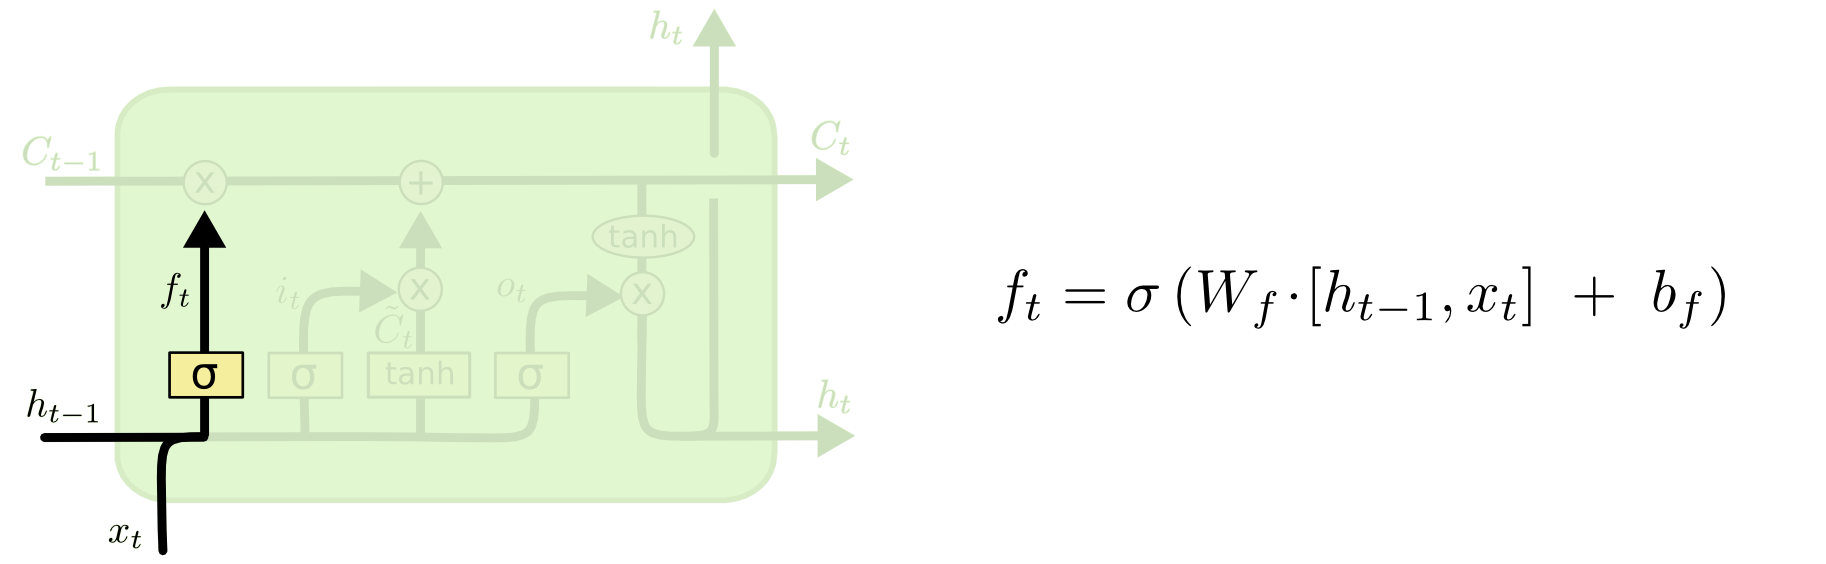
\includegraphics[width=0.65\textwidth]{Images/recurrent_neural_networks/20.png}
  \caption{First, decide what information we’re going to throw away from the cell state}
\end{figure}

\paragraph*{Second} Decide what new information we’re going to store in the cell state. This has two parts. First, a sigmoid layer called the ``input gate layer” decides which values we’ll update. Next, a \textit{tanh} layer creates a vector of new candidate values, $\widetilde{C}_t$, that could be added to the state. In the next step, we’ll combine these two to create an update to the state. For example, in the example of our language model, we’d want to add the gender of the new subject to the cell state, to replace the old one we’re forgetting.

\begin{figure}[h]
  \centering
  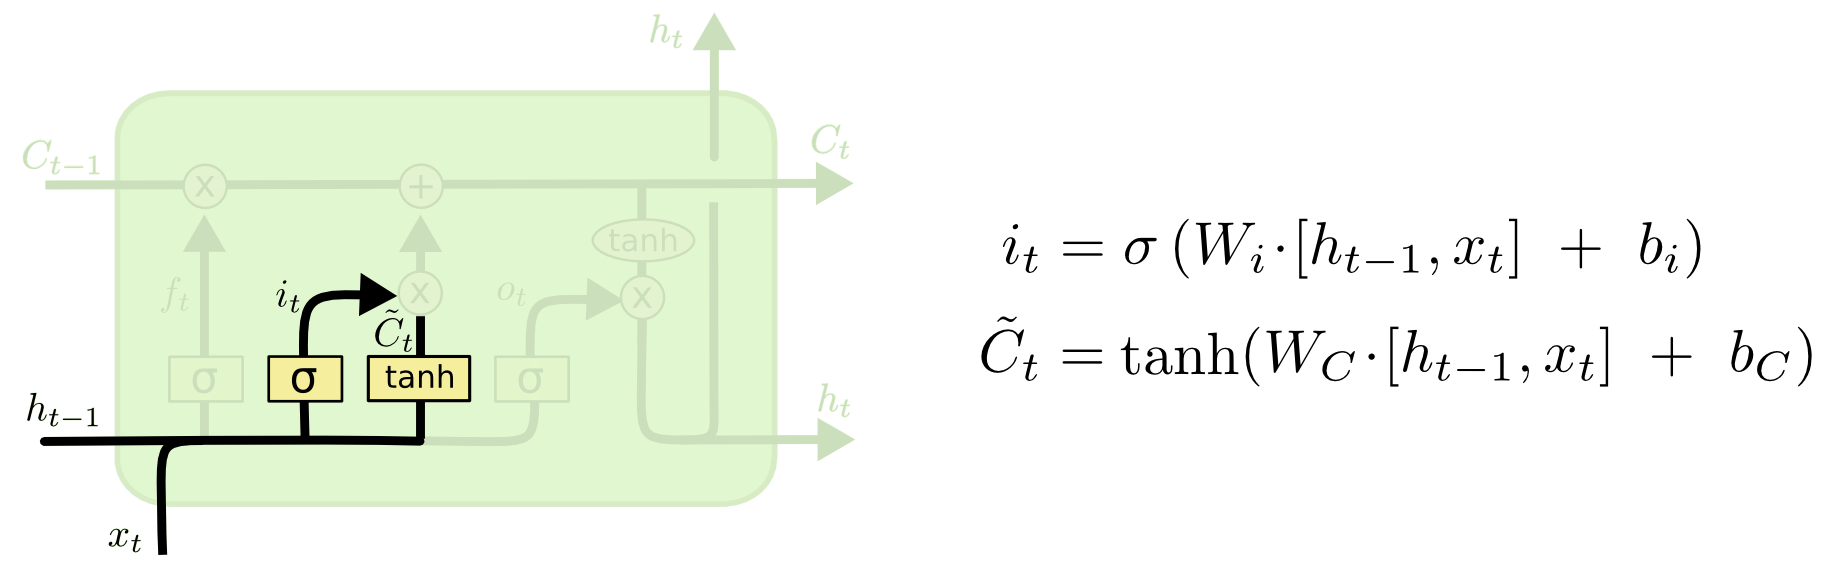
\includegraphics[width=0.65\textwidth]{Images/recurrent_neural_networks/21.png}
  \caption{Second, decide what information we’re going to store in the cell state}
\end{figure}

\paragraph*{Third} Update the old cell state, $C_{t−1}$, into the new cell state CtCt. The previous steps already decided what to do, we just need to actually do it. We multiply the old state by $f_t$, forgetting the things we decided to forget earlier. Then we add $i_t∗\widetilde{C}_t$. This is the new candidate values, scaled by how much we decided to update each state value. In the case of the language model, this is where we’d actually drop the information about the old subject’s gender and add the new information, as we decided in the previous steps.

\begin{figure}[h]
  \centering
  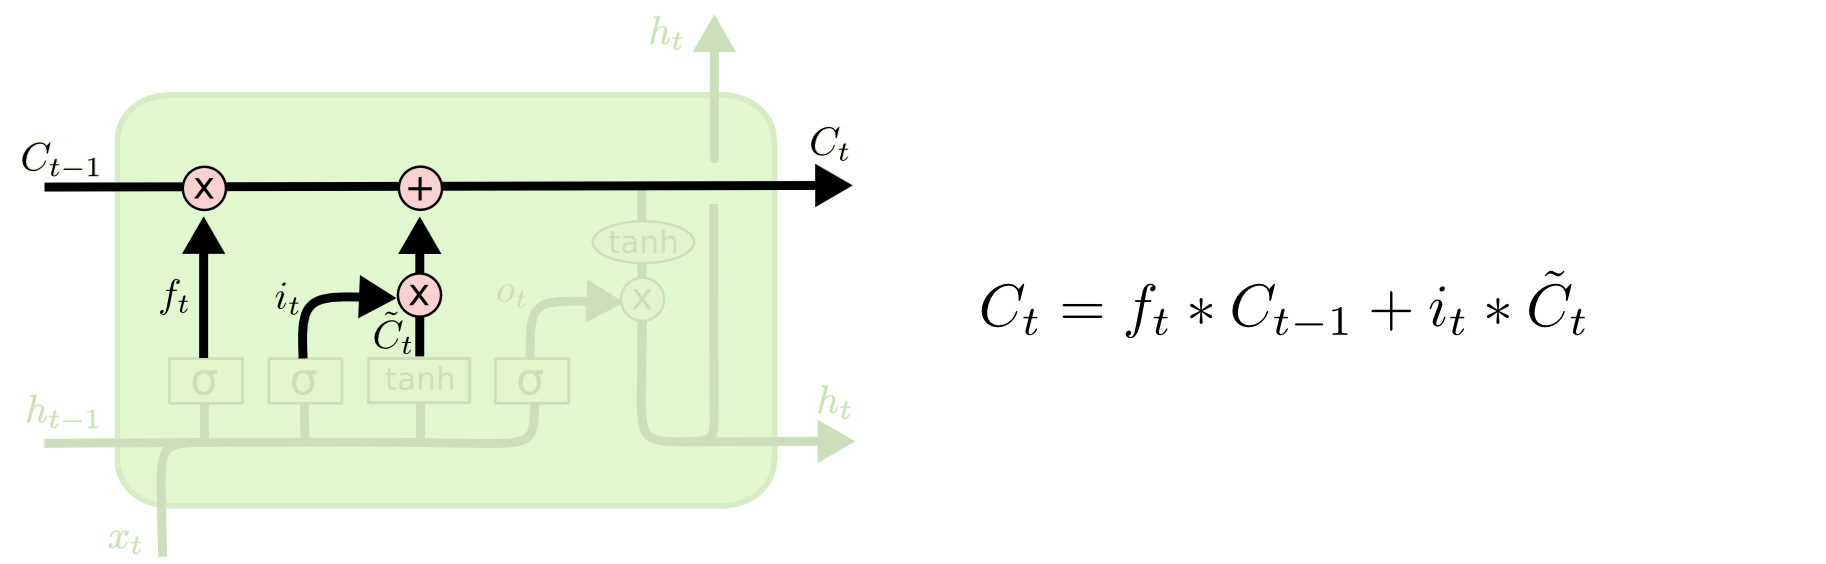
\includegraphics[width=0.65\textwidth]{Images/recurrent_neural_networks/22.png}
  \caption{Third, update the old cell state}
\end{figure}

\paragraph*{Fourth} Finally, we cide what we’re going to output. This output will be based on our cell state, but will be a filtered version. First, we run a sigmoid layer which decides what parts of the cell state we’re going to output. Then, we put the cell state through \textit{tanh} (to push the values to be between $−1$ and $1$) and multiply it by the output of the sigmoid gate, so that we only output the parts we decided to. For the language model example, since it just saw a subject, it might want to output information relevant to a verb, in case that’s what is coming next. For example, it might output whether the subject is singular or plural, so that we know what form a verb should be conjugated into if that’s what follows next.

\begin{figure}[h]
  \centering
  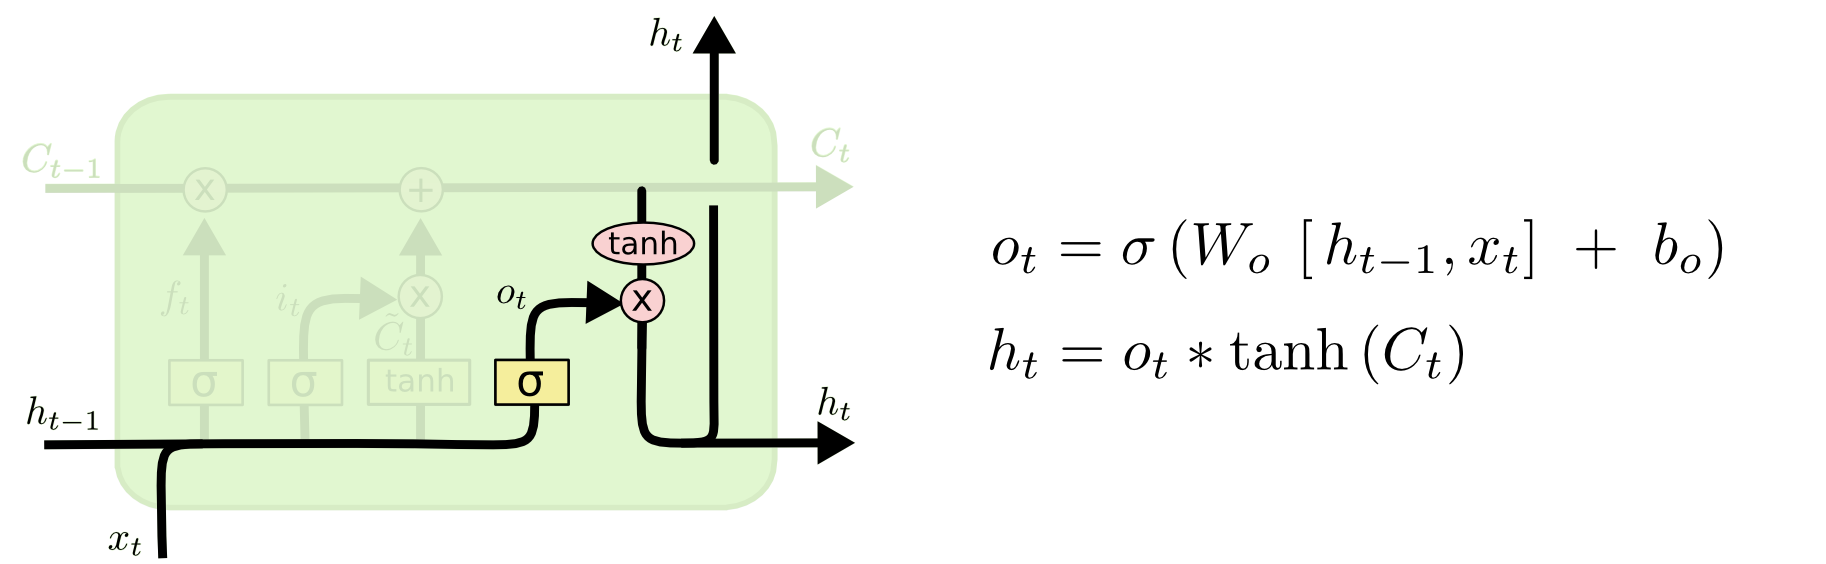
\includegraphics[width=0.65\textwidth]{Images/recurrent_neural_networks/23.png}
  \caption{Fourth, decide what we’re going to output}
\end{figure}

\subsection*{Variants on LSTMs}
But not all LSTMs are the same as the above. In fact, it seems like almost every paper involving LSTMs uses a slightly different version. The differences are minor, but it’s worth mentioning some of them. Greff, et al. (2015) do a nice comparison of popular variants, finding that they’re all about the same.

\begin{figure}[h]
  \centering
  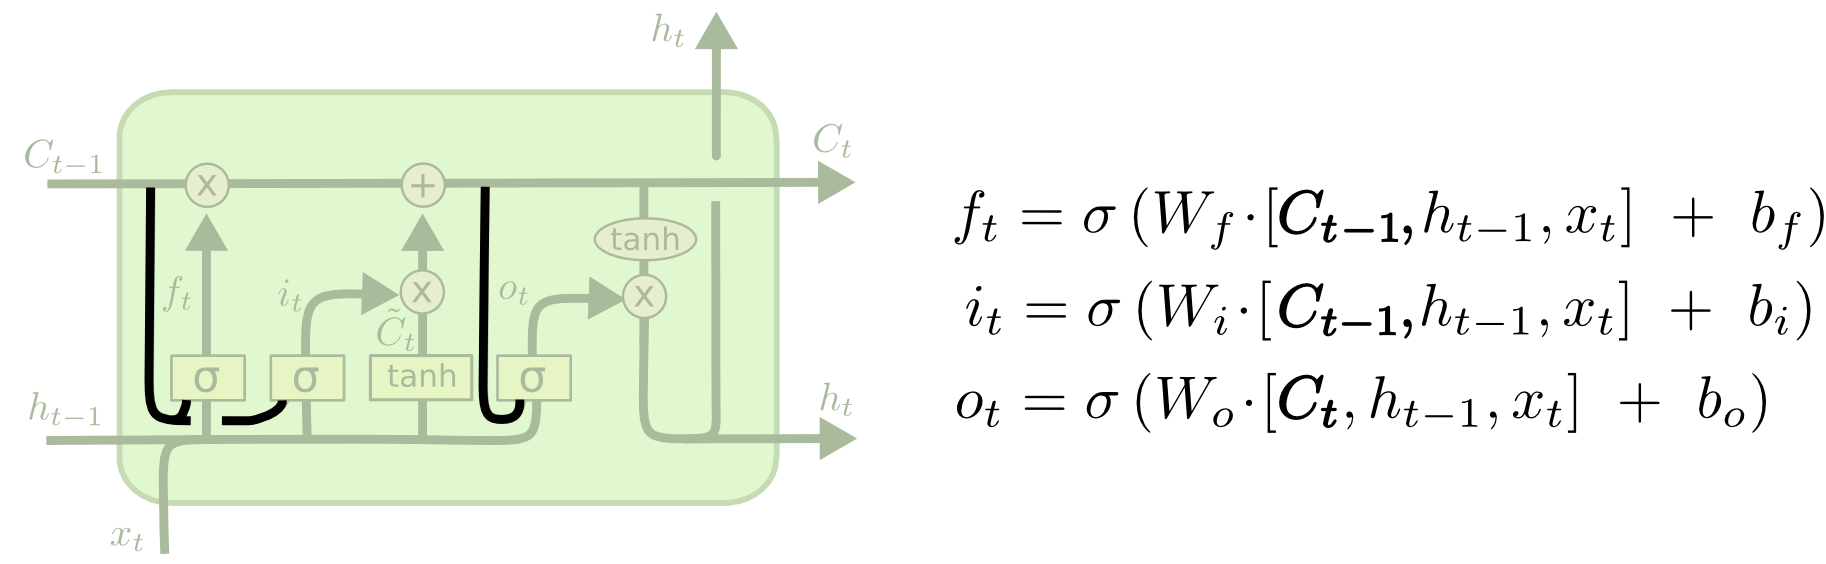
\includegraphics[width=0.65\textwidth]{Images/recurrent_neural_networks/25.png}
  \caption{One popular LSTM variant, introduced by Gers \& Schmidhuber (2000), is adding ``peephole connections.” This means that we let the gate layers look at the cell state. The diagram adds peepholes to all the gates, but many papers will give some peepholes and not others.}
\end{figure}

\begin{figure}[h]
  \centering
  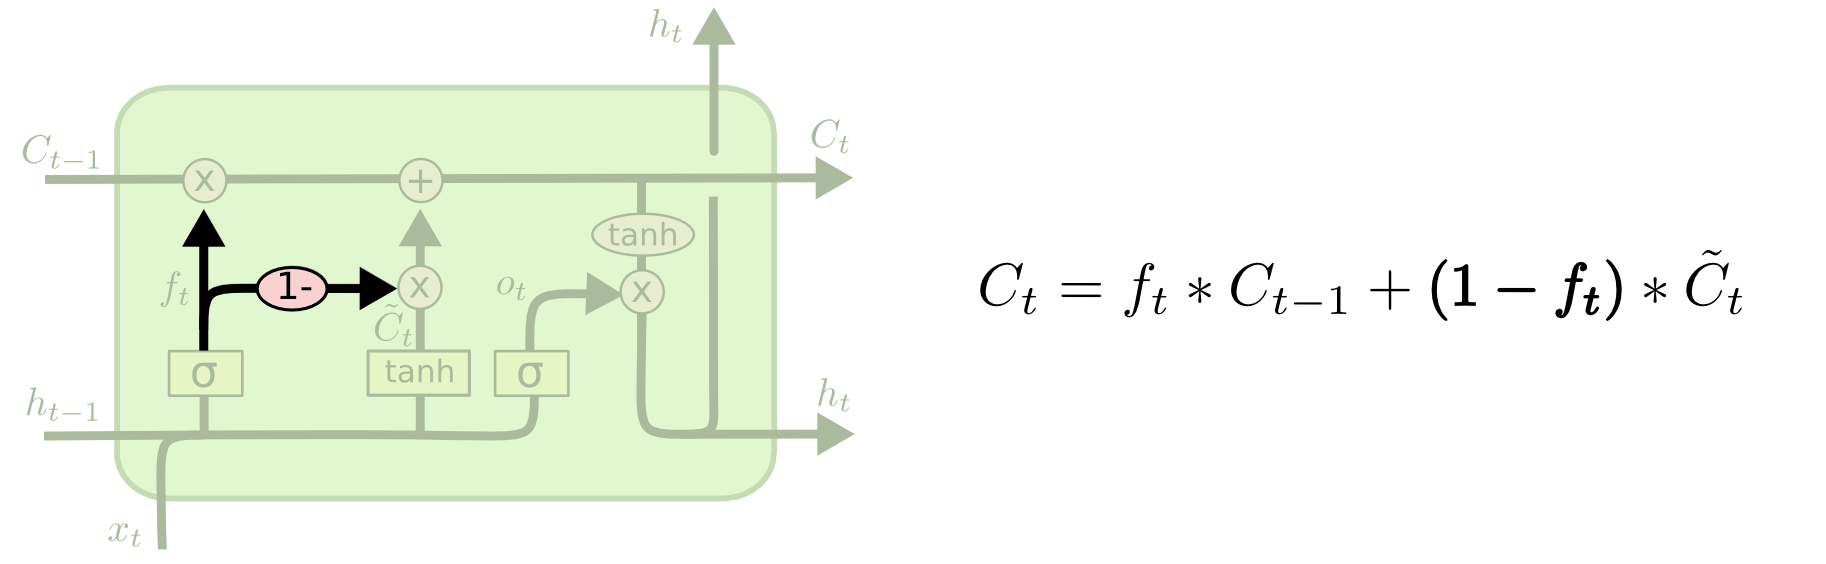
\includegraphics[width=0.65\textwidth]{Images/recurrent_neural_networks/26.png}
  \caption{Another variation is to use coupled forget and input gates. Instead of separately deciding what to forget and what we should add new information to, we make those decisions together. We only forget when we’re going to input something in its place. We only input new values to the state when we forget something older.}
\end{figure}

\begin{figure}[h]
  \centering
  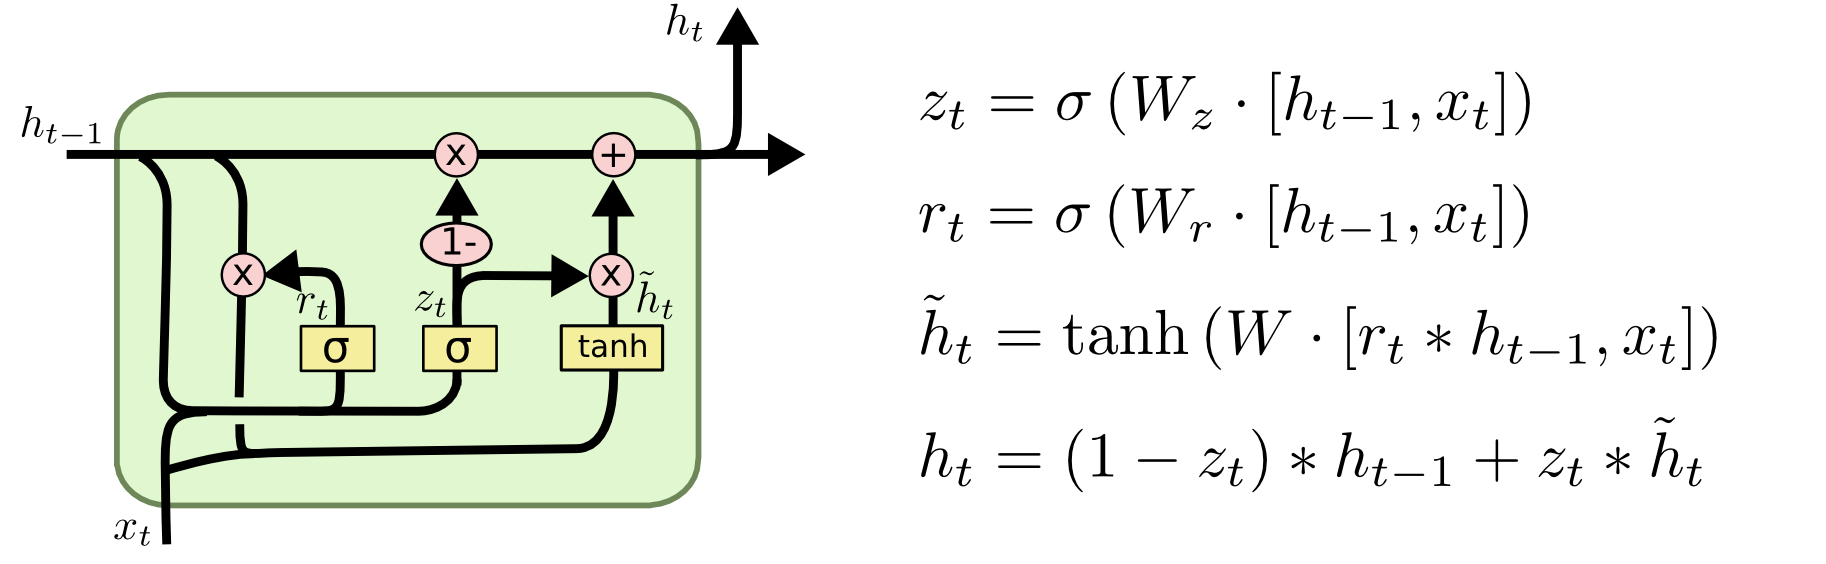
\includegraphics[width=0.65\textwidth]{Images/recurrent_neural_networks/27.png}
  \caption{A slightly more dramatic variation on the LSTM is the Gated Recurrent Unit, or GRU, introduced by Cho, et al. (2014). It combines the forget and input gates into a single ``update gate.” It also merges the cell state and hidden state, and makes some other changes. The resulting model is simpler than standard LSTM models, and has been growing increasingly popular.}
\end{figure}

These are only a few of the most notable LSTM variants. There are lots of others, like Depth Gated RNNs by Yao, et al. (2015). There’s also some completely different approach to tackling long-term dependencies, like Clockwork RNNs by Koutnik, et al. (2014).

\subsection*{Difference between RNN and LSTM}
\begin{figure}[!htb]
  \centering
  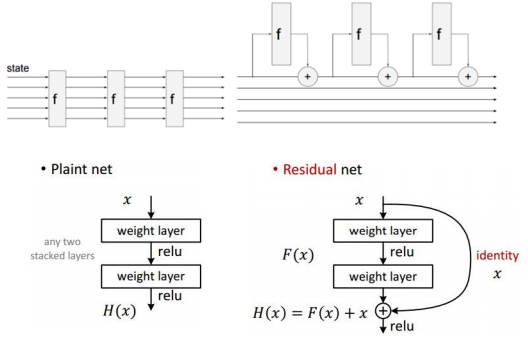
\includegraphics[width=0.65\textwidth]{Images/recurrent_neural_networks/19.png}
  \caption{Difference between RNN (\textbf{left}) and LSTM (\textbf{right})}
\end{figure}

\begin{itemize}
\item RNN transformative interaction of the state, LSTM additive interaction of the state.
\item In RNN you are operating and transforming the state vector. So you are changing your hidden state from time step to time step. Instead, LSTM has these cells states flowing through. A subset of cells (or all of them) to compute the hidden state. Then, based on hidden state, we decide how to operate over the cell. We can reset it and/or adding interaction.
\item RNNs look identical to plain nets, LSTMs to ResNets.
\item RNNs has vanishing gradients, so you can not learn dependencies between distant time steps.LSTMs do not have the problem of vanishing gradients. In a video in evernote they introduce gradient noise to a layer and show how it evolves. We can see that RNN automatically kills it while LSTM maintains it more time. This means that RNN can not learn long term relationships.
\end{itemize}

\subsection{Bidirectional RNN}
A Bidirectional Recurrent Neural Network is a type of Neural Network that contains two RNNs going into different directions. The forward RNN reads the input sequence from start to end, while the backward RNN reads it from end to start. The two RNNs are stacked on top of each others and their states are typically combined by appending the two vectors. Bidirectional RNNs are often used in Natural Language problems, where we want to take the context from both before and after a word into account before making a prediction.


\section*{Summary}
\begin{itemize}
\item RNNs allow a lot of flexibility in architecture design
\item Vanilla RNNs are simple but don’t work very well
\item Common to use LSTM or GRU: their additive interactions improve gradient flow
\item Backward flow of gradients in RNN can explode or vanish. Exploding is controlled with gradient clipping. Vanishing is controlled with additive interactions (LSTM)
\item Better/simpler architectures are a hot topic of current research
\item Better understanding (both theoretical and empirical) is needed.
\end{itemize}


 